\section{Architecture}
\label{architecture}

\begin{figure}[lb]
%\vspace*{-5mm}
\centering
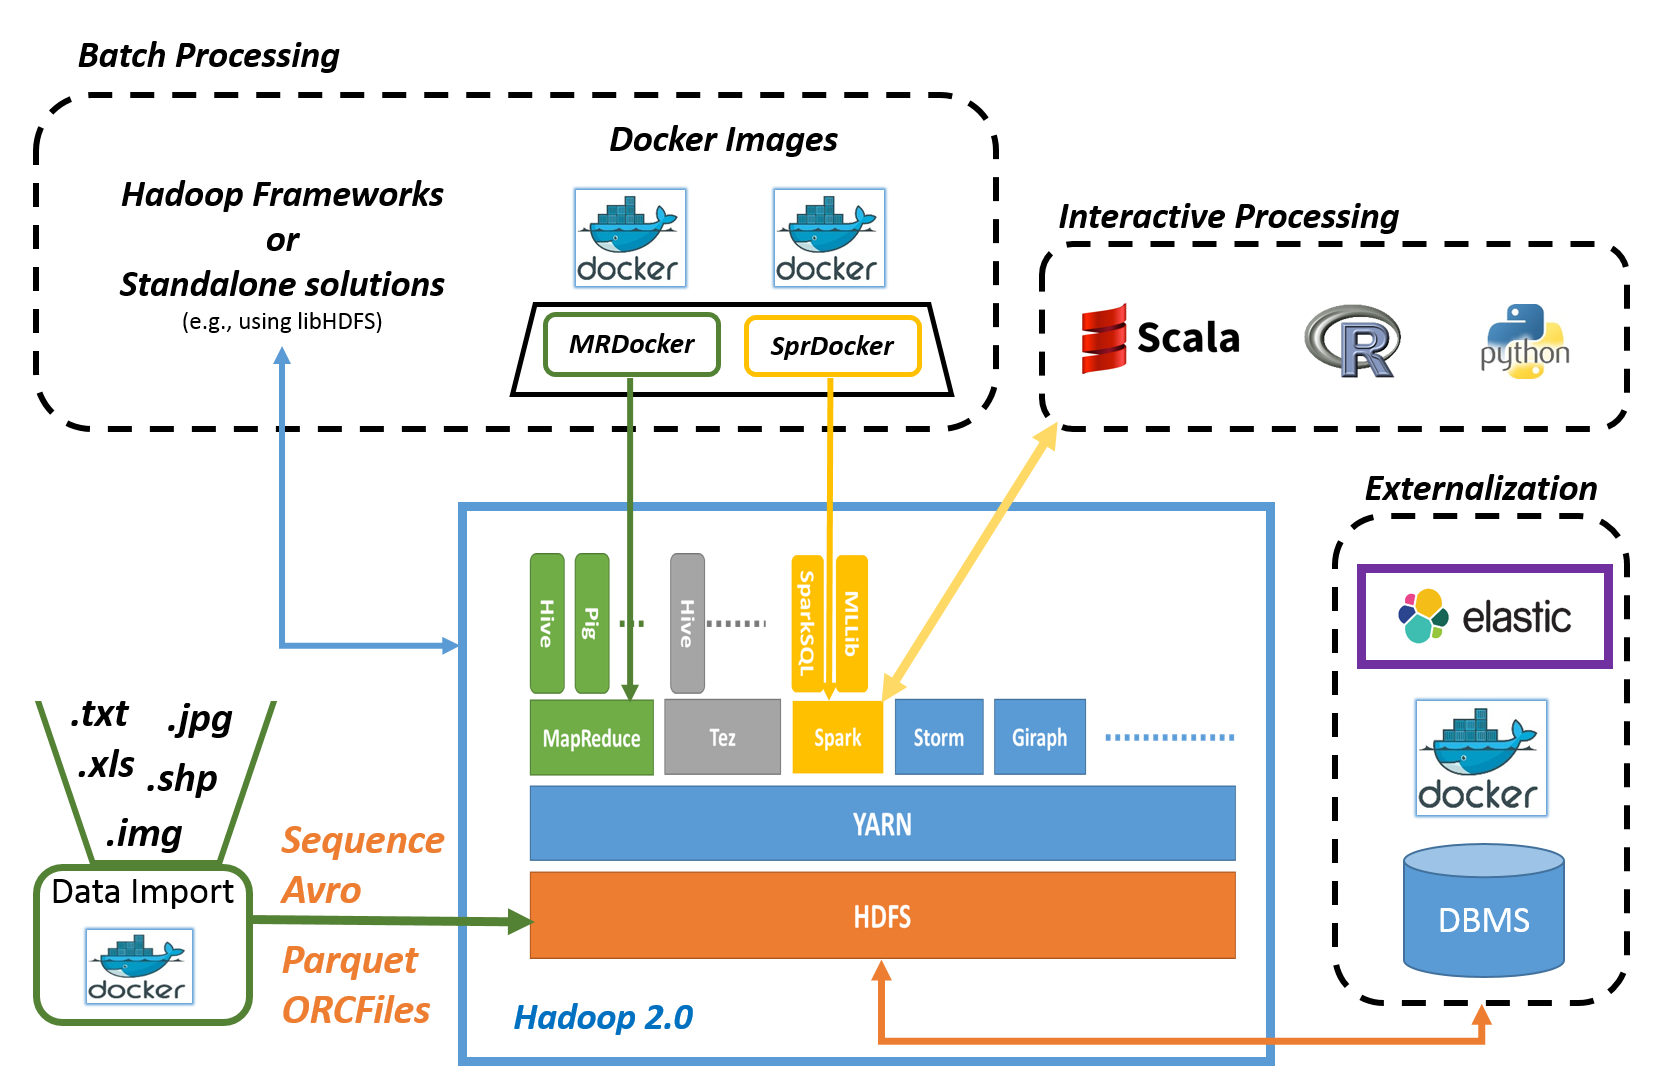
\includegraphics[width=.48\textwidth]{fig/diagram_2.png}
\caption{Data and Tools Integration}
\label{architecture}
\end{figure}

Different state-of-the-art technologies are used to encapsulate and interlink each component in an efficient manner.
Through Docker containers each library and all the context on which it depends is wrapped into a light virtual
image, i.e., a Docker container. Through this technology the library is easily deployed on different platforms.

\subsection{Data Import}
Different type of files will be imported using a Data Import container.

Small files
Avoid data fragmentation
Expose file metadata, scientific data sets are rich in metadata.

In the context of Hansken, HDFS is used as the data hub. On each step of the processing pipe-line each
tool consumes input data stored in HDFS and the outputs the result back to HDFS to be visualized or simply
re-used by other tools. Hence, to exploit data locality, have balanced resource utilization and fault-tolerance,
the Hadoop 2.0 infra-structure is used to schedule and execute Docker instances over data stored in in HDFS.

Ofcourse, you can just copy your files using `hdfs fs -put` commands.
However, this will quickly lead to performance issues on the HDFS filesystem when you have a large number of files (fi. when each file is a twitter message)
You can reduce the number of files by archiving (and zipping) them, but this makes reading them from your spark job difficult.
To get the most out of HDFS, you need to store your data in a format that is a 'Resilient Distributed Dataset' or RDD.
An RDD consists of a set of records with, depending on the format, extensible metadata.
A RDD is split or joined automatically along the records for processing on the hadoop cluster.
This will allow you to use all features like data locality, job scheduling etc.
For optimal performance, it is recommended to convert your data to small number of large RDD files.

\subsubsection{ASCII formats}
For text data, JSON and XML like formats cannot be split at arbitrary places (ie. you need the pair of opening and closing tags for XML to stay valid).
CSV or record JSON, where each line of the file is an independent record, is highly recommended.

General text data can also be converted to a number of binary formats: AVRO, ORC, Parquet, and Sequence files.
A binary file can hold multiple records, which facilitates dealing with large datasets, and some formats
allow you to apply compression.
Other considerations are:

* amount of metadata
* extensability of the the metadata schema: can you add extra fields without having to reimport all data?
* Optimizations on searching on columns
* Support for the format: Hive only, hadoop native, ...
* Availability of supporting tools

AVRO and sequence files are easiest to work with, have native Hadoop support, and usable command line tools exist.
They are not a column store, so performance is slightly lower than the other formats.
ORC seems to become the default format, but support and tooling is still immature.
A combination of AVRO + Parquet seems possible, too.

See the discussion on the following pages:
%<http://www.inquidia.com/news-and-info/hadoop-file-formats-its-not-just-csv-anymore>
%<http://www.slideshare.net/StampedeCon/choosing-an-hdfs-data-storage-format-avro-vs-parquet-and-more-stampedecon-2015>

This link provides an indepth discussion on data practices, considering other aspects than performance and filesize:
%<http://www.confluent.io/blog/stream-data-platform-2/>

and some more blogposts:
%<http://grepalex.com/2014/05/13/parquet-file-format-and-object-model/>
%<http://blog.cloudera.com/blog/2015/03/converting-apache-avro-data-to-parquet-format-in-apache-hadoop/>
%<http://ms-olap.blogspot.nl/2015/02/hive-file-format-comparison.html>
%<https://www.mapr.com/blog/what-kind-hive-table-best-your-data#.VefqGWxSukq>

\subsubsection{Binary formats}
Support for binary data is very limited, only sequence files are a robust solution at the moment.
AVRO supports fixed-length binary blobs, and the other formats can be used for small binary files with some
tricks (like converting binary to base64 text, expanding the data with a factor of 2. Compression could reduce
some of this overhead.)

Import from
-----------

Import from a Database using Apache Sqoop (<https://sqoop.apache.org/>). 
Apache Sqoop is a tool designed for efficiently transferring bulk data between Apache Hadoop and structured
datastores such as relational databases. You can use Sqoop to import data from external structured datastores
into Hadoop Distributed File System or related systems like Hive and HBase. Conversely, Sqoop can be used to
extract data from Hadoop and export it to external structured datastores such as relational databases and
enterprise data warehouses. %Requires a full hdfs installation to work.
%RDMS ↔ Sequence files / AVRO files

Import from binary Files using forqlift (<http://www.exmachinatech.net/projects/forqlift/>).
Commandline tool to work with sequence files File types: text, compressed text, BytesWritable ie. any binary
file format. %normal files ↔ Sequence file


Import from Text (JSON, CSV) using Avro since it has Hadoop native support: java and python bindings; Row based,
not optimized for statistics / aggregates over the metadata; Only fixed-size binary blobs.

Avro files are quickly becoming the best multi-purpose storage format within Hadoop. Avro files store
metadata with the data but also allow specification of an independent schema for reading the file. This
makes Avro the epitome of schema evolution support since you can rename, add, delete and change the data
types of fields by defining new independent schema. Additionally, Avro files are splittable, support
block compression and enjoy broad, relatively mature, tool support within the Hadoop ecosystem.

Apache Avro™ is a data serialization system, providing: Rich data structures; A compact, fast, binary
data format; A container file, to store persistent data; Remote procedure call (RPC); Simple integration
with dynamic languages; Code generation is not required to read or write data files nor to use or implement
RPC protocols; Code generation as an optional optimization, only worth implementing for statically
typed languages; From Python: avro, avroknife (pip).


Apache orc, ORC: optimized row columnar can add user metadata per file

ORC is a self-describing type-aware columnar file format designed for Hadoop workloads. It is optimized
for large streaming reads, but with integrated support for finding required rows quickly. Storing data
in a columnar format lets the reader read, decompress, and process only the values that are required
for the current query. Because ORC files are type-aware, the writer chooses the most appropriate encoding
for the type and builds an internal index as the file is written. Predicate pushdown uses those indexes
to determine which stripes in a file need to be read for a particular query and the row indexes can
narrow the search to a particular set of 10,000 rows. ORC supports the complete set of types in Hive,
including the complex types: structs,


Apache Parquet, a columnar storage format
Apache Parquet is a columnar storage format available to any project in the Hadoop ecosystem, regardless
of the choice of data processing framework, data model or programming language.

\subsection{Batch Processing}

\subsubsection{MapReduce}
The first wave of Mappers will be slow because they will have to download the libraries for each Docker
instance. However, such image is then cached. We need to configure dockter to not use too much space
and thus clean the cache once new type of instances are run.

As first step towards a Map-Docker function was implemented deployed using MapReduce processing paradigm.
Such function runs a simple Docker instance using a Java "System call" and through Hadoop streaming API
it reads from stdin and writes to the stdout. The second option is to explore the Docker Java API to
implement more advanced options to load input data and output the results, but also to start and stop
the Docker instance. A set of templates on how to do it can be found at hadoop-streaming-docker.

\subsubsection{Spark}
In search for efficiency, the second step was to deploy Docker instances using Spark on the same YARN
cluster. After setting up a SPARK cluster, using the following instructions, the deployment of Spark
jobs was studied in the context of Latent Dirichlet Allocation (LDA) which is part of the machine learn
library of Spark. LDA is used by the topic modeling team to classify emails by topic. To use LDA
efficiently the input data was re-structured into a SequenceFile archives using Forqlift. With the
data stores as SequenceFile archives the data preparation phase of LDA takes advantage of data locality
and uses all the available resources.

To run a Docker instance a spark app called \emph{spark\_docker} was developed. All the instructions
on how to run Docker from a Spark app can be found at spark-docker. The \emph{spark\_docker} was tested
in the context of image classification. The library uses neural networks to classify a set of images
and it was developed by the deep learning group. Using a Docker image stored at DockerHub, \emph{spark\_docker}
instantiated one per node which used as input the local images and outputted into a CSV file the name
of the file and the classification result. Such final result is then readable by the visualization layer
using the NFS mount.

How to do it for HDFS cluster, we run docker containers in Spark.
When using HDFS, better to use Spark because data locality comes for free.

In Spark 1.2, we’ve taken the next step to allow Spark to integrate natively with a far larger number
of input sources.  These new integrations are made possible through the inclusion of the new Spark SQL
Data Sources API.

https://databricks.com/blog/2015/01/09/spark-sql-data-sources-api-unified-data-access-for-the-spark-platform.html


\subsection{Interactive Processing}

\subsubsection{Python}

\subsubsection{R-enviroment}

\subsection{Externalization}
Furthermore, to make all the files stored in HDFS accessible as POSIX two options were considered: FUSE
and NFS. With both solutions HDFS will be mounted as a directory to be provided as input to the Docker
instance. After trying both options, NFS seems to be easier to setup and used by a larger user community.

\subsubsection{Database Management System}

Such initial stage could be seen as a data gathering stage where data parallelism is evident.

An option is to use a files directly by a DBMS.
For data we are also working on data vaults\cite{ivanova13}.
Drop the text.

Database with Hadoop integration such has BigSQL 3.0 and Polybase.

Impala which can then process Parquet files.


\subsubsection{External services}
Elastic Search

Web-services through docker containers.


